\documentclass[11pt,letterpaper]{article}
\usepackage[T1]{fontenc}
\usepackage[scaled]{helvet}
\renewcommand{\familydefault}{\sfdefault}
\usepackage{amsmath,amssymb}
\usepackage[margin=0.8in,bottom=0.9in]{geometry}
\usepackage[most]{tcolorbox}
\usepackage{tikz}
\usetikzlibrary{calc}
\usepackage{enumitem}
\usepackage{array}
\usepackage{needspace}
\usepackage{fancyhdr}
\usepackage{pifont}

% ---- Palette "F. Bright & Playful" ----
\definecolor{fmtitle}{HTML}{3D2C8D}
\definecolor{fmkey}{HTML}{0096C7}
\definecolor{fmwatch}{HTML}{2BB673}
\definecolor{fmturn}{HTML}{F4A100}
\definecolor{fmmistake}{HTML}{EF476F}
\definecolor{fmnotice}{HTML}{9B5DE5}
\definecolor{fmgray}{HTML}{6B6B6B}

\pagestyle{fancy}
\fancyhf{}
\renewcommand{\headrulewidth}{0pt}
\fancyfoot[C]{\footnotesize\color{fmgray}\textcopyright\ 2026 FangMath. All rights reserved.}
\fancyfoot[R]{\footnotesize\color{fmgray}\thepage}
\setlength{\parindent}{0pt}
\setlength{\parskip}{3pt}

\newcommand{\badge}[1]{\colorbox{fmtitle}{\color{white}\bfseries\small\ #1\ }}
\newcommand{\leveltag}[2]{\colorbox{#1}{\color{white}\bfseries\scriptsize\ #2\ }}
\newcommand{\LE}{\leveltag{fmwatch}{EASY}}
\newcommand{\LM}{\leveltag{fmturn}{MEDIUM}}
\newcommand{\LH}{\leveltag{fmmistake}{HARD}}

\newcommand{\sectionbar}[2]{\needspace{6cm}\par\vspace{4mm}
  \begin{tcolorbox}[enhanced,colback=fmtitle,colframe=fmtitle,arc=2mm,
    left=4mm,top=1.5mm,bottom=1.5mm]
  \color{white}\bfseries\large #1\hfill{\normalsize\mdseries #2}
  \end{tcolorbox}}

\newtcolorbox{keyidea}{enhanced,breakable,colback=white,colframe=fmkey,boxrule=1pt,arc=2mm,
  title={Key Idea},coltitle=fmkey,fonttitle=\bfseries,
  attach boxed title to top left={xshift=4mm,yshift=-2mm},
  boxed title style={colback=white,colframe=fmkey,boxrule=0.9pt}}
\newtcolorbox{watchme}{enhanced,colback=white,colframe=fmwatch,boxrule=1pt,arc=2mm,
  title={Watch Me --- Worked Example},coltitle=fmwatch,fonttitle=\bfseries,
  attach boxed title to top left={xshift=4mm,yshift=-2mm},
  boxed title style={colback=white,colframe=fmwatch,boxrule=0.9pt}}
\newtcolorbox{mistakebox}{enhanced,breakable,colback=white,colframe=fmmistake,boxrule=1pt,arc=2mm,
  title={Common Mistake},coltitle=fmmistake,fonttitle=\bfseries,
  attach boxed title to top left={xshift=4mm,yshift=-2mm},
  boxed title style={colback=white,colframe=fmmistake,boxrule=0.9pt}}
\newtcolorbox{yourturn}{enhanced,breakable,colback=white,colframe=fmturn,boxrule=1pt,arc=2mm,
  title={Your Turn},coltitle=fmturn,fonttitle=\bfseries,
  attach boxed title to top left={xshift=4mm,yshift=-2mm},
  boxed title style={colback=white,colframe=fmturn,boxrule=0.9pt}}
\newtcolorbox{answerbox}[1]{enhanced,breakable,colback=white,colframe=fmwatch,boxrule=1pt,arc=2mm,
  title={#1},coltitle=fmwatch,fonttitle=\bfseries,
  attach boxed title to top left={xshift=4mm,yshift=-2mm},
  boxed title style={colback=white,colframe=fmwatch,boxrule=0.9pt}}

\newcommand{\work}[1]{\par\vspace{#1}}
\setlist[enumerate]{itemsep=2pt,topsep=3pt}

% ---------------- extra boxes ----------------
\newtcolorbox{notebox}{enhanced,breakable,colback=white,colframe=fmnotice,boxrule=1pt,arc=2mm,
  title={Notice},coltitle=fmnotice,fonttitle=\bfseries,
  attach boxed title to top left={xshift=4mm,yshift=-2mm},
  boxed title style={colback=white,colframe=fmnotice,boxrule=0.9pt}}
\newtcolorbox{exbox}{enhanced,colback=white,colframe=fmwatch,boxrule=0.8pt,arc=2mm,
  title={Example},coltitle=fmwatch,fonttitle=\bfseries\small,
  attach boxed title to top left={xshift=4mm,yshift=-2mm},
  boxed title style={colback=white,colframe=fmwatch,boxrule=0.8pt},fontupper=\small}
\newcommand{\topicbar}[1]{\needspace{4.5cm}\par\vspace{5mm}
  \begin{tcolorbox}[enhanced,colback=fmtitle,colframe=fmtitle,arc=2mm,left=4mm,top=1.5mm,bottom=1.5mm]
  \color{white}\bfseries\large #1
  \end{tcolorbox}}
\usepackage{multicol}

% ---------------- practice layout ----------------
\newcommand{\workline}{\par\vspace{7mm}{\color{gray!55}\rule{\linewidth}{0.4pt}}}
\newcommand{\worklines}[1]{\foreach \i in {1,...,#1}{\workline}}
\newcommand{\prob}[3]{\needspace{#3}\par\vspace{3mm}{\color{fmturn}\bfseries #1.}\ #2\par}
\newcommand{\ansline}{\par\vspace{4mm}\hfill\textbf{Answer:}\ \rule{5cm}{0.4pt}\par}
\newcommand{\keyitem}[3]{\needspace{3.2cm}\par\vspace{2mm}
  \begin{tcolorbox}[enhanced,colback=white,colframe=fmwatch!60,boxrule=0.6pt,arc=1.5mm,left=3mm,top=1.5mm,bottom=1.5mm]
  {\color{fmwatch}\bfseries #1.}\quad\small #2\par\vspace{1mm}
  \normalsize\textbf{Answer: #3}
  \end{tcolorbox}}


\usetikzlibrary{arrows.meta}
\providecommand{\iskey}{0}
% fill-in blank: line for students, pink answer in the key
\newcommand{\fb}[2][2.6cm]{\ifnum\iskey=1 \underline{\makebox[#1][c]{\color{fmmistake}\bfseries #2}}\else\underline{\makebox[#1]{}}\fi}
% answer line for practice problems
\newcommand{\pans}[2][3.2cm]{\ifnum\iskey=1 \underline{\makebox[#1][c]{\color{fmmistake}\bfseries #2}}\else\rule{#1}{0.4pt}\fi}
\newcommand{\vid}[1]{\needspace{5.2cm}\par{\color{fmgray}\small\textit{\ding{43} Video: #1}}}
\newcommand{\pt}[2]{\fill (#1) circle (2.2pt) node[above=1pt,font=\small]{$#2$};}

\usetikzlibrary{decorations.pathreplacing}

\usetikzlibrary{arrows.meta}
% parallel lines l, m cut by transversal t; #1 = comma list of angle numbers to highlight
\newcommand{\tfig}[1][]{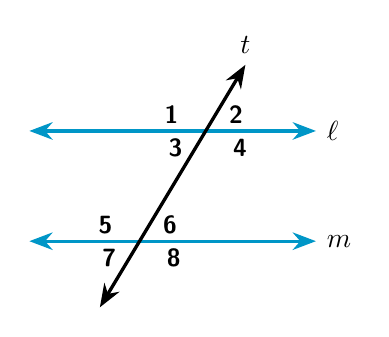
\begin{tikzpicture}[scale=0.7]
\draw[very thick,fmkey,{Stealth}-{Stealth}] (-2.6,1)--(2.6,1) node[right,black]{$\ell$};
\draw[very thick,fmkey,{Stealth}-{Stealth}] (-2.6,-1)--(2.6,-1) node[right,black]{$m$};
\draw[very thick,{Stealth}-{Stealth}] (-1.32,-2.2)--(1.32,2.2) node[above]{$t$};
\foreach \n/\x/\y in {1/-0.02/1.3,2/1.15/1.3,3/0.05/0.7,4/1.22/0.7,5/-1.22/-0.7,6/-0.05/-0.7,7/-1.15/-1.3,8/0.02/-1.3}{\node[font=\small\bfseries] at (\x,\y){\n};}
\end{tikzpicture}}
\begin{document}
\ifnum\iskey=1 \colorbox{fmwatch}{\color{white}\bfseries\small\ ANSWER KEY\ }\else\badge{WATCH \& FILL IN}\fi\hfill{\small\color{fmgray}Geometry \textperiodcentered\ Lesson 3.3}\par\vspace{4mm}
{\color{fmtitle}\LARGE\bfseries Proving Lines Parallel --- Notes\ifnum\iskey=1 \ --- Answer Key\fi}\par\vspace{1mm}
{\color{fmgray}Watch the video and fill in each blank. Pause when you see ``Your turn.''}\par\vspace{3mm}
Name: \rule{6cm}{0.4pt}\hspace{1cm}Date: \rule{3.5cm}{0.4pt}\par\vspace{2mm}


\vid{Run it backwards}
\begin{keyidea}Last lesson: lines parallel $\Rightarrow$ angles congruent.\par\vspace{1mm}
This lesson: angles congruent $\Rightarrow$ \fb[2.4cm]{lines parallel}. \ These are called \fb[2cm]{converses}.\end{keyidea}

\vid{The converses}
\begin{keyidea}\begin{minipage}[c]{0.3\linewidth}\centering\tfig\end{minipage}\hfill
\begin{minipage}[c]{0.64\linewidth}\renewcommand{\arraystretch}{1.6}\begin{tabular}{@{}l@{}}
\fb[3cm]{Corresponding} angles congruent $\Rightarrow \ell \parallel m$\\
Alt.\ interior \textbf{or} alt.\ exterior angles \fb[2.2cm]{congruent} $\Rightarrow \ell \parallel m$\\
Same-side interior angles \fb[3cm]{supplementary} $\Rightarrow \ell \parallel m$\\
Two lines parallel to the \fb[1.4cm]{same} line are parallel.\\
\end{tabular}\end{minipage}\end{keyidea}

\vid{Prove it}
\begin{watchme}$m\angle 4 = 72^\circ$, \ $m\angle 5 = 72^\circ$. \ Is $\ell \parallel m$?\par\vspace{1mm}
\renewcommand{\arraystretch}{1.6}\begin{tabular}{@{}l l@{}}
1.\ Name the pair: & \fb[3.4cm]{alternate interior}\\
2.\ Same measure, so & $\angle 4 \cong \angle 5$\\
3.\ So $\ell \parallel m$ by the & \fb[6cm]{Alternate Interior Angles Converse}\\
\end{tabular}\end{watchme}

\vid{Find $x$ so the lines are parallel}
\begin{watchme}Same-side interior: $(4x + 6)^\circ$ and $(5x - 15)^\circ$.\par\vspace{1mm}
Need a \fb[1.4cm]{sum} of $180^\circ$: \ $9x - 9 = 180$ \ $\Rightarrow$ \ $x = $ \fb[1.2cm]{$21$}\end{watchme}

\vid{Watch out}
\begin{mistakebox}Never use ``they \fb[2.2cm]{look parallel}.'' Name the angle pair, show it is congruent (or supplementary), then name the \fb[2cm]{converse}.\end{mistakebox}

\vid{Your turn}
\begin{yourturn}$m\angle 1 = 115^\circ$, \ $m\angle 8 = 115^\circ$. Is $\ell \parallel m$? Which converse?\par\vspace{2mm}
$\angle 1$ and $\angle 8$ are \fb[3.4cm]{alternate exterior} angles, and they are congruent.\par\vspace{1mm}
$\ell \parallel m$? \fb[1.2cm]{yes} \quad by the \fb[6cm]{Alternate Exterior Angles Converse}\end{yourturn}

\begin{notebox}\textbf{Remember:}\quad Congruent corresponding or alternate angles $\Rightarrow$ parallel.\quad Supplementary same-side interior angles $\Rightarrow$ parallel.\quad Name the pair, show the angle fact, name the converse.\end{notebox}
\end{document}
